\documentclass{article}
%Some packages I commonly use.
\usepackage[english]{babel}
\usepackage{graphicx}
\usepackage{framed}
\usepackage[normalem]{ulem}
\usepackage{amsmath}
\usepackage{amsthm}
\usepackage{amssymb}
\usepackage{amsfonts}
\usepackage{enumerate}
\usepackage[utf8]{inputenc}
\usepackage[left = 1in, right = 1in, top = 1in, bottom= 1in]{geometry}
\usepackage{amsmath}
\usepackage{esvect}
\usepackage{enumitem}
\usepackage{textcomp}
\usepackage{float}
\usepackage{siunitx}

\usepackage{array}
\usepackage{wrapfig}
\usepackage{multirow}
\usepackage{tablefootnote}
\usepackage{threeparttable}
\usepackage{tabularx} % allows text wrap in tables
\usepackage{subcaption}
    \setlength{\captionmargin}{25pt}
\usepackage{makecell}

%A bunch of definitions that make my life easier
\newcommand{\matlab}{{\sc Matlab} }
\newcommand{\cvec}[1]{{\mathbf #1}}
\newcommand{\rvec}[1]{\vec{\mathbf #1}}
\newcommand{\ihat}{\hat{\textbf{\i}}}
\newcommand{\jhat}{\hat{\textbf{\j}}}
\newcommand{\khat}{\hat{\textbf{k}}}
\newcommand{\minor}{{\rm minor}}
\newcommand{\trace}{{\rm trace}}
\newcommand{\spn}{{\rm Span}}
\newcommand{\rem}{{\rm rem}}
\newcommand{\ran}{{\rm range}}
\newcommand{\range}{{\rm range}}
\newcommand{\mdiv}{{\rm div}}
\newcommand{\proj}{{\rm proj}}
\newcommand{\R}{\mathbb{R}}
\newcommand{\N}{\mathbb{N}}
\newcommand{\Q}{\mathbb{Q}}
\newcommand{\Z}{\mathbb{Z}}
\newcommand{\<}{\langle}
\renewcommand{\>}{\rangle}
\renewcommand{\emptyset}{\varnothing}
\newcommand{\attn}[1]{\textbf{#1}}
\theoremstyle{definition}
\newtheorem{theorem}{Theorem}
\newtheorem{corollary}{Corollary}
\newtheorem*{definition}{Definition}
\newtheorem*{example}{Example}
\newtheorem*{note}{Note}
\newtheorem{exercise}{Exercise}
\newcommand{\bproof}{\bigskip {\bf Proof. }}
\newcommand{\eproof}{\hfill\qedsymbol}
\newcommand{\Disp}{\displaystyle}
\newcommand{\qe}{\hfill\(\bigtriangledown\)}
\setlength{\columnseprule}{1 pt}


\begin{document}
\noindent{\hfill{\bf{USCLAP Competition 2020-21}}}

\vspace{4cm}

\begin{center}
    \section*{Impact of Opioid Prescription Rate on Suicide Rates and Poverty Levels of Counties in the United States}
        
    \vspace{4cm}
    

\section*{Abstract}
    Opioids continue to flood into our communities through prescriptions from doctors and dentists. In this study, we attempt to determine the relationship between opioid prescription rates of a county and the county’s associated suicide rate and poverty levels. Data was pulled from government websites and compiled into one large data set. The opioid prescription rate was then used as the independent variable to be compared against the other two variables in multiple statistical tests to see if there is a positive correlation between the three variables. All p-values were found to be well below our significance level of $\alpha = 0.05$, all slopes were positive, and all adjusted $R^2$ values were positive as well. Our results suggest that there is a positive relationship between the three analyzed variables—if poverty level is fixed, increasing suicide rates still correlates with increasing opioid prescription rates and vice versa. We hope that this research project will bring greater social awareness to the severity of the opioid crisis and thus prompt greater support and resource distribution efforts at the community level. 
\end{center}

\newpage

\section*{Introduction}
\hspace{\parindent} On August 13th, 2020, NPR published ``Doctors and Dentists Still Flooding U.S With Opioid Prescriptions," which discusses how health care professionals are still prescribing opioids at an alarming rate [3]. This opioid epidemic has plagued our country since the late 1990s, causing widespread misuse and fatal addictions. Furthermore, according to an NIH article, ``Suicide Deaths are a Major Component of the Opioid Crisis that Must be Addressed," some experts believe that up to 30\% of opioid overdoses may actually be suicides [5]. In fact, the strength of the relationship between suicides and opioids have seemed to increase with time, and in a 2017 study, it was shown that people who misused prescription opioids had a much higher rate of suicide ideation, even when controlling for other health conditions[1]. Additionally, those misusing opioid prescriptions were about twice as likely to attempt suicide compared to those that did not misuse opioids [1]. Per these articles and the ongoing opioid crisis, this project looks into the factors that may affect the rate of opioid prescriptions in relation to suicides rates and poverty levels. Specifically, this project attempts to address the question: Is a larger rate of legal opioid prescription related to higher numbers in suicide and poverty rates? Our null hypothesis assumes there is no correlation between opioid prescription rates, suicide rates, and poverty levels. Our one-sided alternate hypothesis checks for a positive correlation between the three variables. 


%%%%

\section*{Methods}
\hspace{\parindent} We used three separate datasets in this project. From the Center for Disease Control and Prevention (CDC) website, we obtained an opioid prescription dataset that provides the number of opioid prescriptions per 100 residents, by state and county, from 2005 to 2015 [6]. We also obtained the suicide dataset from the CDC, which provides the suicide death rates in the United States per county per 100,000 people from 2008 to 2014 [4]. Finally, the poverty dataset is obtained from the Health Resources and Services Administration (HRSA) website. The data includes the percentage of families, by state and county, with incomes below 1.0, 1.5, and 2.0 times the Federal Poverty Level (FPL) from 2014 to 2018 [2]. The independent variable for this project is opioid prescription rates (OPR).  The dependent variables are suicide rates (SR),   poverty index (PI), and the percentages of families below 1 times the Federal Poverty Rate (P1.0), 1.5 times the FPL (P1.5), and 2.0 times the FPL (P2.0). The OPR describes the average opioid prescriptions dispensed per 100 persons in each county. The SR describes death rates (by suicide) per 100,000 people in each county. The P1.0, P1.5, and P2.0 describes the average percentage of families with incomes below 1.0, 1.5, and 2.0 times the FPL, inclusive and grouped by county. The PI is a weighted percentage of people in poverty. This calculated value prevents double counting of people and weights those below the FPL more heavily in each county. This was calculated by taking P1.0 with full weight, P1.50 with $2/3$ weight, P2.00 with $1/3$ weight, and families above P2.00 with no weight. The higher the poverty index, the more families near or in poverty in respective counties. The population in our study is the counties in the U.S., not including territories and provided there is data for all three variables available ($n = 1768$). To conduct our research, we first plotted scatter plots and residual plots, then gathered our test statistic, the slope ($\beta_1$), along with $R^2$,  and p-values from simple regression models: SR, P1.0, P1.5, P2.0, or PI as a function of OPR. Simulations were run for all simple regression models—null permutations of the models (assume no relationship between the independent and dependent variables), null plots with test statistic (See Appendix, Figures 2-6 for reference), null p-values, bootstrap simulations to generate 95\% confidence intervals to show the range in which the test statistic could have been in. We also ran a multiple regression model to compare OPR to the two main dependent variables: SR and PI. After running the models, we made a scatter plot incorporating OPR, SR, and PI to better visualize the relationships between them.



%%%%

\section*{Results}
\hspace{\parindent} Our first question asks whether or not there is a relationship between opioid prescription rates (OPR), suicide rates (SR), and the various poverty statistics we used (P1.0, P1.5, P2.0, PI). If there is a relationship, is it a positive trending relationship?  From our linear regression models, we found that OPR versus all other variables yielded p-values $\num{< 2.26e-16}$, and small, positive slopes and adjusted $R^2$ values (Table 1).


\begin{table}[h]
\centering
\caption{Linear Regression Analysis of Opioids and Other Variables}
\begin{tabular}{|c|c|c|c|c|c|c|}
\hline
\textbf{Model} & \textbf{NDist. p-value} & \textbf{LM p-value} & \textbf{Adj. $R^2$} & \textbf{Slope} & \textbf{LM Slope CI} & \textbf{BTSP CI}\\ \hline 
    OPR x SR & $0$ & $\num{<2.2e-16}$ & $0.061$ & $0.032$ & $(0.026, 0.037)$ & $(0.026, 0.037)$ \\ \hline
    OPR x P1.0 & $0$ & $\num{<2.2e-16}$ & $0.16$ & $0.045$ & $(0.040, 0.050)$ & $(0.039, 0.050)$ \\ \hline
    OPR x P1.5 & $0$ & $\num{<2.2e-16}$ & $0.16$ & $0.067$ & $(0.060. 0.074)$ & $(0.059, 0.075)$  \\ \hline
    OPR x P2.0 & $0$ & $\num{<2.2e-16}$ & $0.16$ & $0.086$ & $(0.077, 0.095)$ & $(0.077, 0.095)$  \\ \hline
    OPR x PI & $0$ & $\num{<2.2e-16}$ & $0.17$ & $0.066$ & $(0.059, 0.073)$ & $(0.059, 0.073)$ \\ \hline
\end{tabular}
\label{tb:decay}
\end{table}

For all the other variables, OPR may be a statistically significant predictor, as the calculated p-values were much smaller than the significance level of $\alpha = 0.05$. The linear model, however, does not seem too practical, as the adjusted $R^2$ values suggest that these models would be less than 20\% accurate for predicting values (Table 1). The null distributions showed that the test statistic slopes were in fact not within the distribution of null slopes (See Appendix, Figures 2-6 for reference). The p-values given from the null permutations were, rounded to the thousandth, 0 for all the models (Table 1). The generated 95\% confidence intervals do not contain 0 and are all in the positive range, indicating a potentially positive relationship. 

In addition to looking at the relationships individually, we obtained a multiple regression model as given below:
\begin{equation*}
    \widehat{OPR} = 25.853	 + 2.320 \times PI + 1.461 \times SR 
\end{equation*}
This model accounts for the two major explanatory variables—PI and SR—and indicates that a 0.1 increase in PI is associated with a 23 opioid prescription increase per 100 people, after accounting for SR. Similarly, a 1 person increase in SR is associated with a .00001461 opioid prescription increase per 100 people, after accounting for PI. From our analysis, there is statistically significant evidence that both PI and SR are associated with an increase in OPR, as the p-value for both the variables in the regression model, the model as a whole, is 0. 

\begin{figure}[H]
    \centering
    \includegraphics[height = 8.25cm]{SPO.pdf}
    \caption{Scatter plot of opioid prescription rate versus suicide rate, color coded with a gradient of our calculated poverty index. The higher the poverty index, the more poverty in the county, as represented in red. The median poverty counties are represented by white dots, and the low poverty counties are represented in green. The points on this plot have been jittered to avoid too much overlap of points.}
    \label{fig:my_label}
\end{figure} 


To better visualize the relationship between the variables, OPR and SR were plotted and colored by PI (Figure 1). While the lower portion of PI is grouped over the lower left portion of the scatter plot, the upper portion of the gradient is well spread from the low end of OPR to the high end. The counties with the lowest PI also appear to place lower on SR, while the very low and very high SR have moderate to high PI. This further suggests some positive relationship between OPR, SR, and PI. 


%%%%
\section*{Discussion}
\hspace{\parindent} Based on our findings above, we can reject our null hypothesis that there is no relationship between opioid prescription rate (OPR), suicide rate (SR), and poverty (PI), and accept our one-sided alternative that there is a positive relationship between the three variables. This conclusion was drawn from 5 different linear regression so OPR versus dependent variables and from a multiple regression analysis of OPR versus SR and PI. All of the higher prescription rate counties are counties of above the moderate poverty index, and we can see that most of the lower poverty counties stop at around 1 prescription per person (which is still very high), showing a clear relationship between wealth and prescription rate. We also see that many of the darker red (higher PI counties) are at the low and high ends of opioid prescriptions. This discrepancy is addressed below. However, our findings also demonstrated that this relationship is very weak, as indicated by adjusted $R^2 = 0.0608$ from OPR versus SR, $R^2 = 0.1652$ from OPR versus PI, and $R^2 = 0.198$ from the multiple regression model. 

One important limitation worth mentioning is the exploration of several simple regression models comparing OPR to various dependent variables. A much lower significance level could have been used to avoid the Fallacy of Multiple Testing, but as the p-values were 0 when rounded to the thousandth, we kept it at $\alpha = 0.05$. With more code, more significant figures could have been drawn out and can be look at for further research. The dependent variables themselves might also have strong correlations that explain some of the variation observed in the data.  Using the multiple linear regression model with OPR and SR + PI as inputs in the model, we were able to further explore this relationship and investigate how OPR influences SR, while controlling for PI.

Furthermore, there were many limitations to our dataset. Using poverty indexes or brackets of the FPL to determine a family's well-being can be misleading. A family's income may not necessarily tell us all about the family's living situation or living standards. For example, current income does not take into consideration liquid assets, savings, debt, credit, goods or services that may be obtained with things other than income (gifts, exchanges, etc.), government services or financial aid. Thus, by only using income as a measure of poverty, we may be misrepresenting parts of population that are defined as living in poverty but are not actually poor. Additionally, we do not take into account how healthcare access varies from region to region. This may also be misleading since areas with higher opioid prescription rates may be higher simply because they have more doctors to prescribe them opioids. Likewise, areas with lower prescription rates may be lower because they have fewer (or no) doctors to prescribe them opioids. Of course, this is only considering that the population is obtaining opioids in a legal manner. This brings us to another limitation of our dataset–the data does not account for illegally distributed opioids. For example, in areas where there is high illegal opioid activity, there may be low legal opioid prescriptions because the opioids are being obtained in a different manner. There are some limitations in our suicide dataset as well. Our suicide dataset does not take into account suicide attempts unless the attempts result in death, nor does it take into account suicide ideation. This may provide an incomplete picture of suicidal behavior in relation to opioid prescriptions. Additionally, gathering data on suicides may be difficult due to inconsistencies in defining what constitutes a suicide. 

A limitation of this project itself is that we only looked at how opioid prescription rates affected suicide rates, and not other diseases. However, this limitation does not necessarily indicate that relationships between opioid prescription rates and other severe illnesses, such as depression, do not exist. The opioid crisis is devastating and has consequences that may be associated with a vast number of other illnesses. Thus, it is crucial for future work to look into ways of ending opioid addition. Despite the vast limitations of our dataset and this project, acknowledging that these relationships exist is an important step in addressing these issues.  By conducting more research on this topic and the potential factors that affect opioid prescription rates, we can better understand where the issue is coming from and thus address it properly. For example, future work could look into the benefits of redistributing resources in under-served communities where opioid addiction is prevalent. 


\section*{References}
    \begin{enumerate}[label={[\arabic*]}]
     \item Ashrafioun, Lisham, Todd M. Bishop, Kenneth R. Conner, and Wilfred R. Pigeon. ``Frequency of Prescription Opioid Misuse and Suicidal Ideation, Planning, and Attempts.” \textit{Journal of Psychiatric Research} 92 (September 1, 2017): 1–7. https://doi.org/10.1016/j.jpsychires.2017.03.011.
    \item ``Data Explorer.” Accessed August 13, 2020. https://data.hrsa.gov/tools/data-explorer?ds=29,34.
    \item NPR.org. ``Doctors And Dentists Still Flooding U.S. With Opioid Prescriptions.” Accessed August 13, 2020. https://www.npr.org/2020/07/17/887590699/doctors-and-dentists-still-flooding-u-s-with-opioid-prescriptions.
    \item ``F MapF Mapping Module.” Accessed August 13, 2020. https://wisqars.cdc.gov:8443/cdcMapFramework/mapModuleInterface.jsp.

    \item NIMH ``Suicide Deaths Are a Major Component of the Opioid Crisis That Must Be Addressed.” Accessed August 13, 2020. https://www.nimh.nih.gov/about/director/messages/2019/suicide-deaths-are-a-major-component-of-the-opioid-crisis-that-must-be-addressed.shtml.
    \item ``U.S. Opioid Prescribing Rate Maps | Drug Overdose | CDC Injury Center,” March 12, 2020. https://www.cdc.gov/drugoverdose/maps/rxrate-maps.html.

    \end{enumerate}

\newpage

\section*{Appendix}
\begin{figure}[H]
    \centering
    \includegraphics[height = 9cm]{SR_OPR.pdf}
    \caption{Suicide rate and opioid prescription rate graphs for analyzing linear model. 
}
    \label{fig:my_label}
\end{figure} 

\begin{figure}[H]
    \centering
    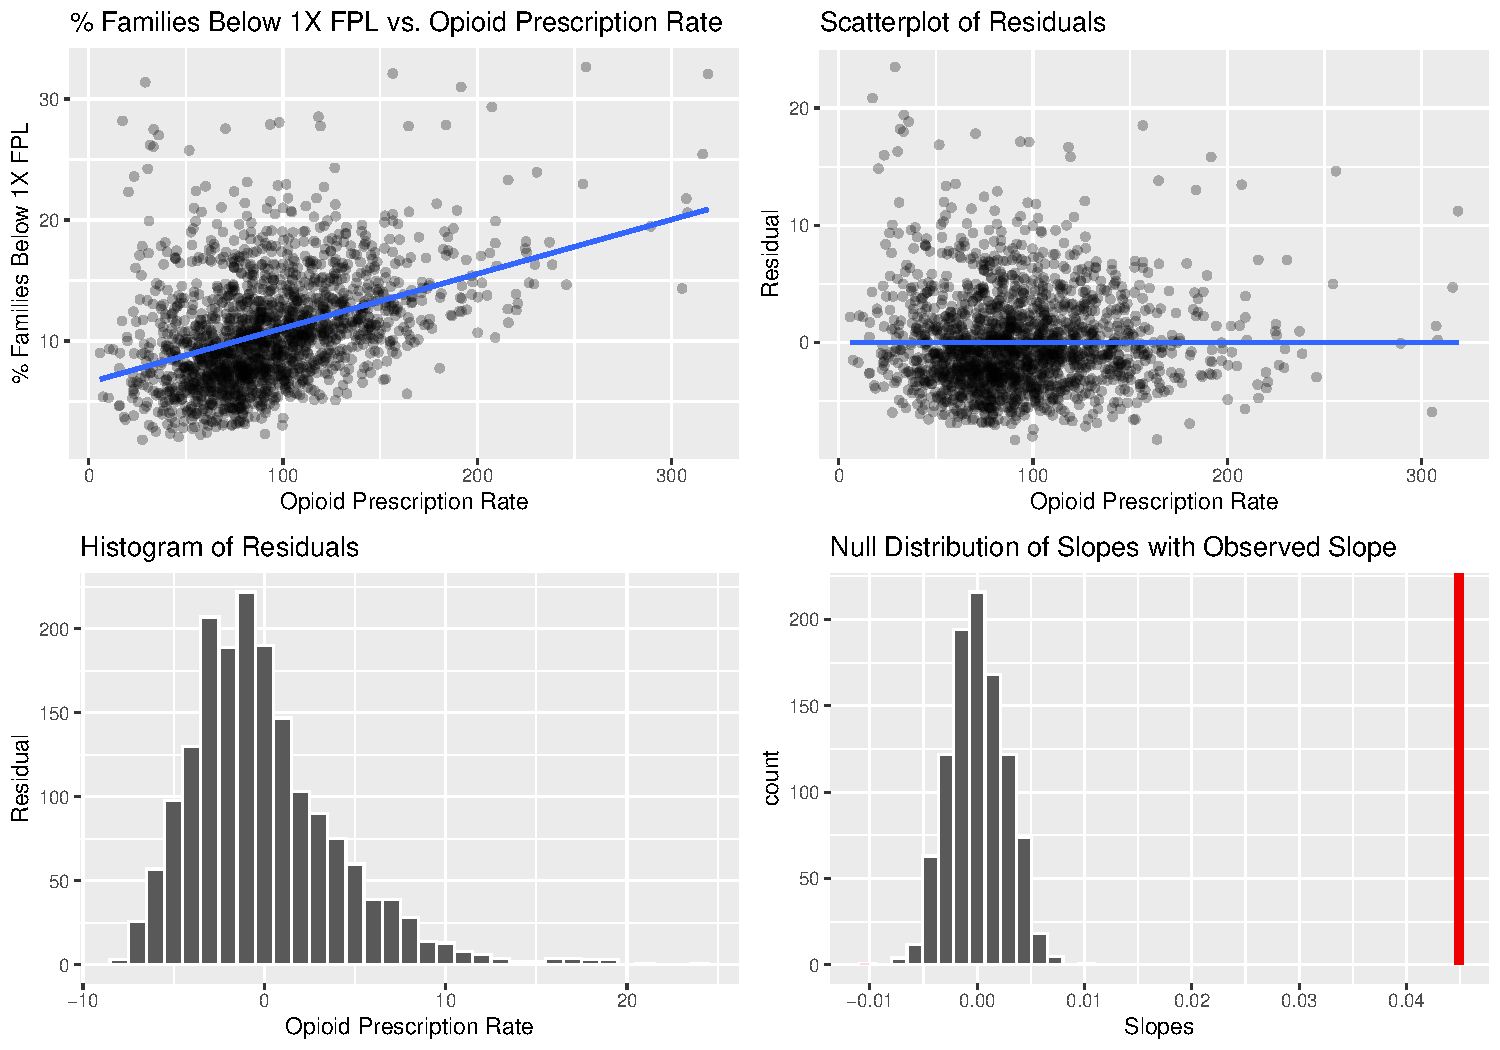
\includegraphics[height = 9cm]{P1_OPR.pdf}
    \caption{Percentage of families with incomes below 1.0x FPL and opioid prescription rate graphs for analyzing linear model.
}
    \label{fig:my_label}
\end{figure} 

\begin{figure}[H]
    \centering
    \includegraphics[height = 9cm]{P1_5_OPR.pdf}
    \caption{Percentage of families with incomes below 1.5x FPL and opioid prescription rate graphs for analyzing linear model.
}
    \label{fig:my_label}
\end{figure} 

\begin{figure}[H]
    \centering
    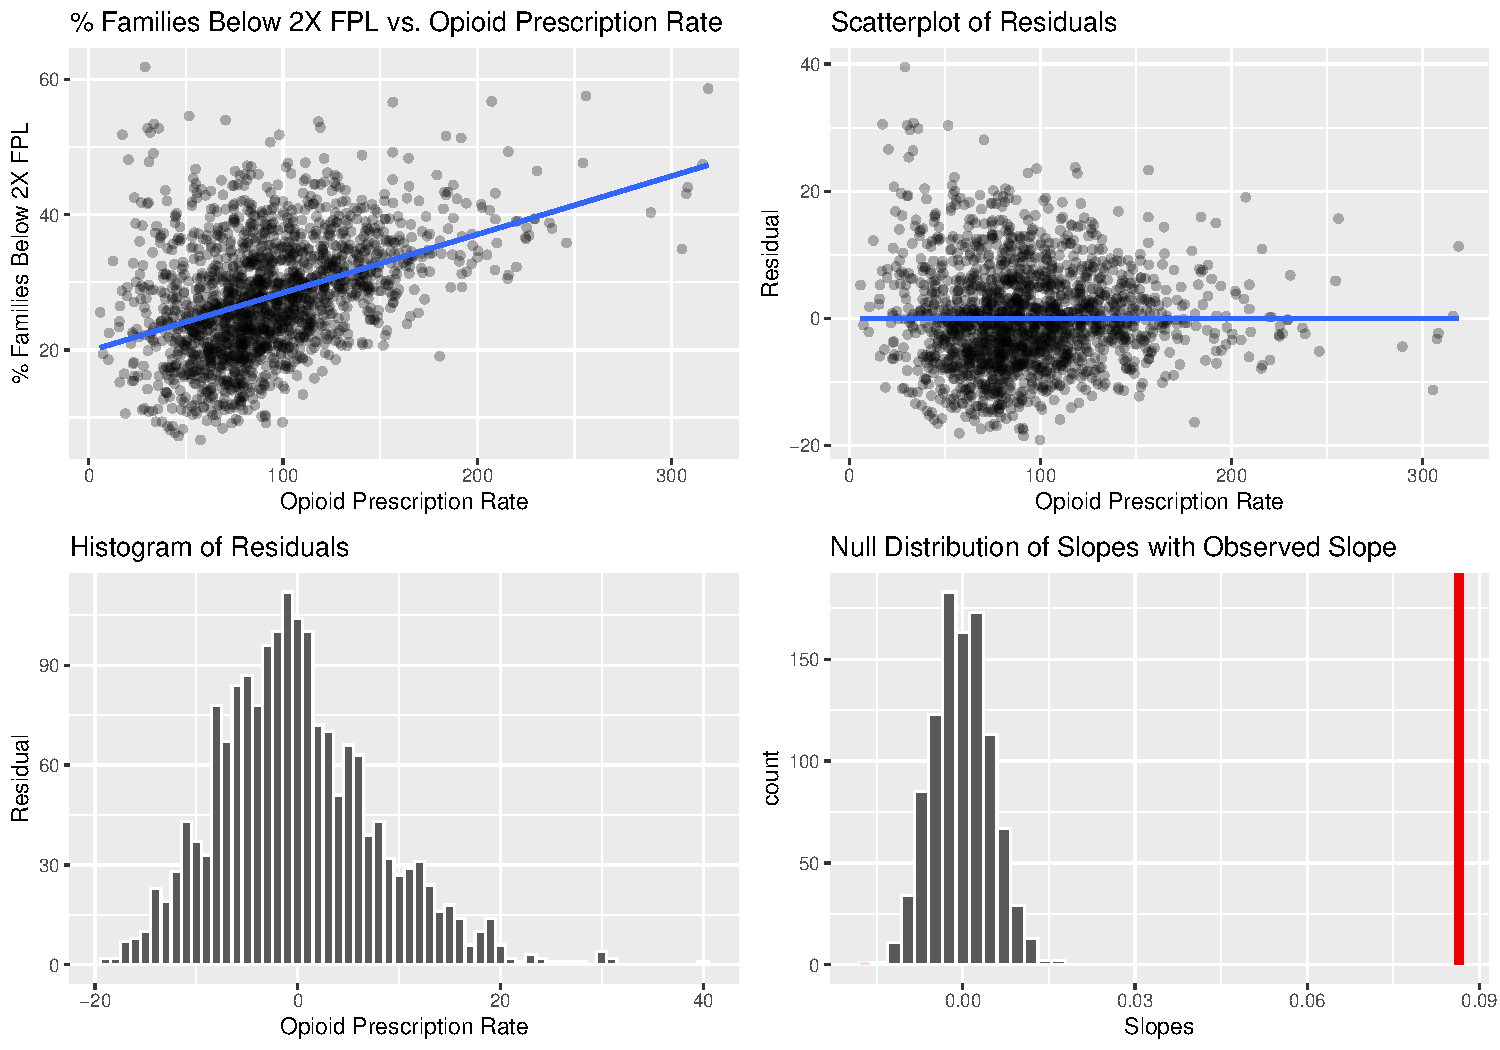
\includegraphics[height = 9cm]{P2_OPR.pdf}
    \caption{Percentage of families with incomes below 2.0x FPL and opioid prescription rate graphs for analyzing linear model.
}
    \label{fig:my_label}
\end{figure}
\begin{figure}[H]
    \centering
    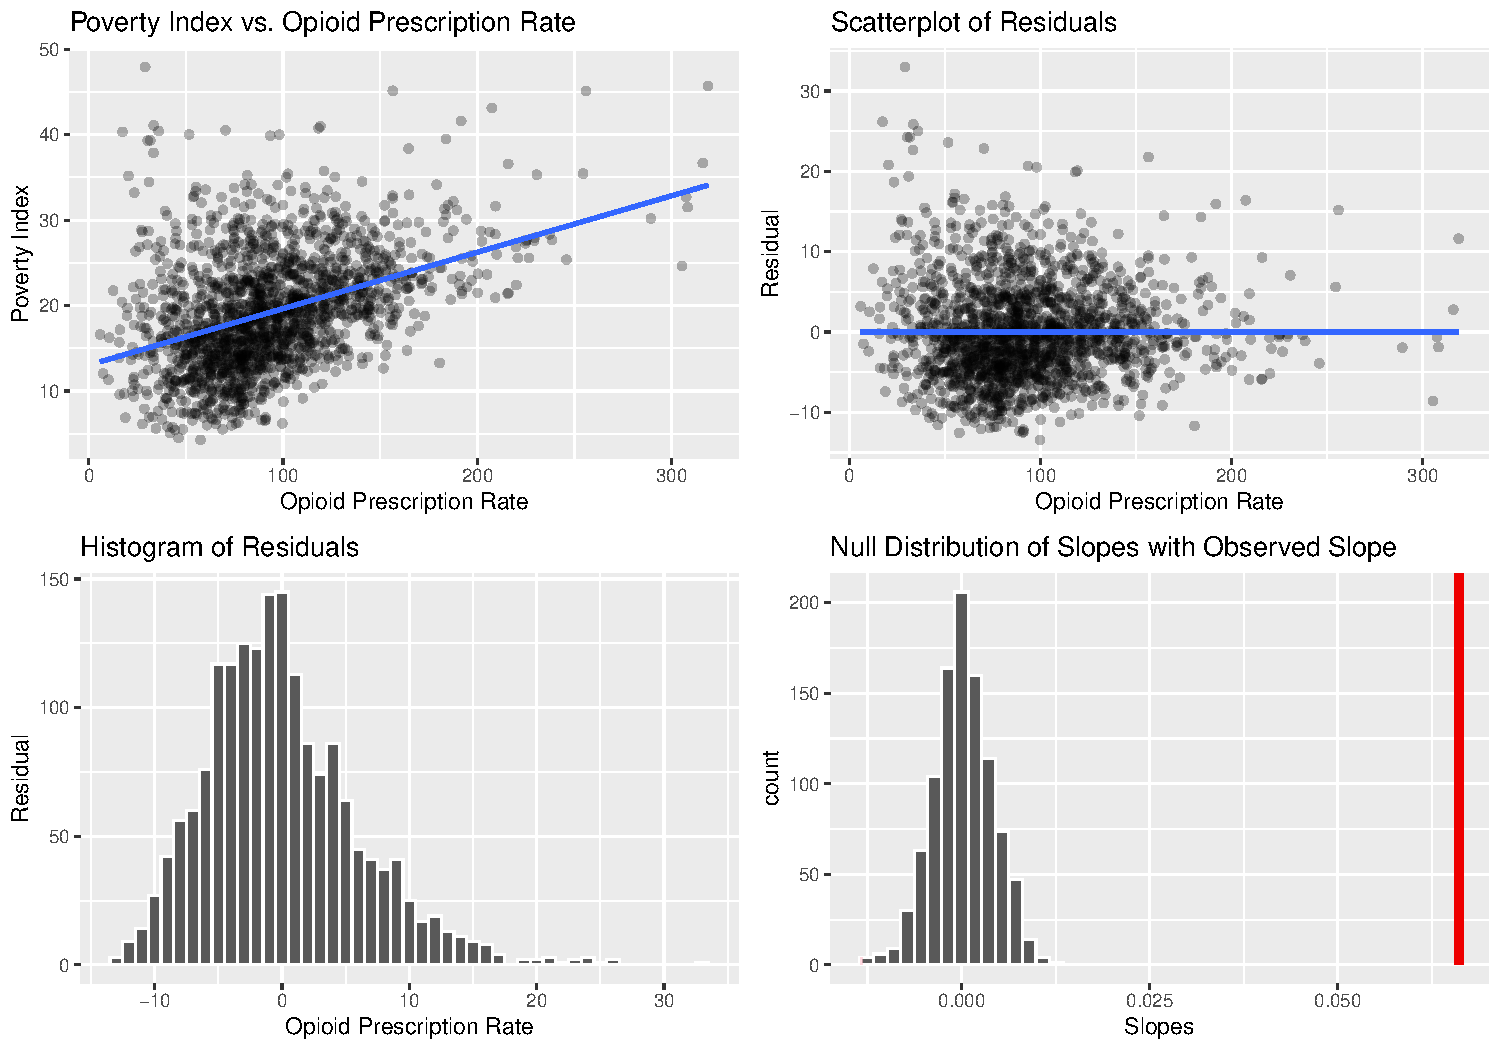
\includegraphics[height = 9cm]{PI_OPR.pdf}
    \caption{Poverty Index and opioid prescription rate graphs for analyzing linear model.
}
    \label{fig:my_label}
\end{figure}
\begin{figure}[H]
    \centering
    \includegraphics[height = 9cm]{SR_PI.pdf}
    \caption{Poverty Index and Suicide Rate graphs for analyzing linear model to observe relationship not directly studied.
}
    \label{fig:my_label}
\end{figure}
\end{document}